\documentclass{standalone}

\usepackage{tikz}
\usepackage{amsfonts}
\usetikzlibrary{positioning, mindmap, shadows, shapes}

\begin{document}
\begin{tikzpicture}

\path[mindmap,
    text = white,
    every node/.style = {
      concept,
      circular drop shadow
    },
    root/.style = {
      concept color = red!40,
      font = \Large\bfseries, 
      text width = 8em
    },
    level 1 concept/.append style = {
      concept color = blue!40,
      font = \Large\bfseries,
      sibling angle = 120,
      text width = 8em,
      level distance = 15em,
      inner sep = 0pt
    },
    level 2 concept/.append style = {
      concept color = purple!60,
      font = \bfseries\Huge,
      sibling angle = 20,
      text width = 7em,
      level distance = 14em
    },
    level 3 concept/.append style = {
      concept color = violet,
      font = \bfseries\Huge,
      sibling angle = 60,
      text width = 5em,
      level distance = 10em
    },
  ]
  node[root] {Set \\ Theory} [counterclockwise from = 210]
    child[] {
      node {A Branch of Mathematics} [clockwise from = -90]
	child [] {node (cantor) [rectangle] {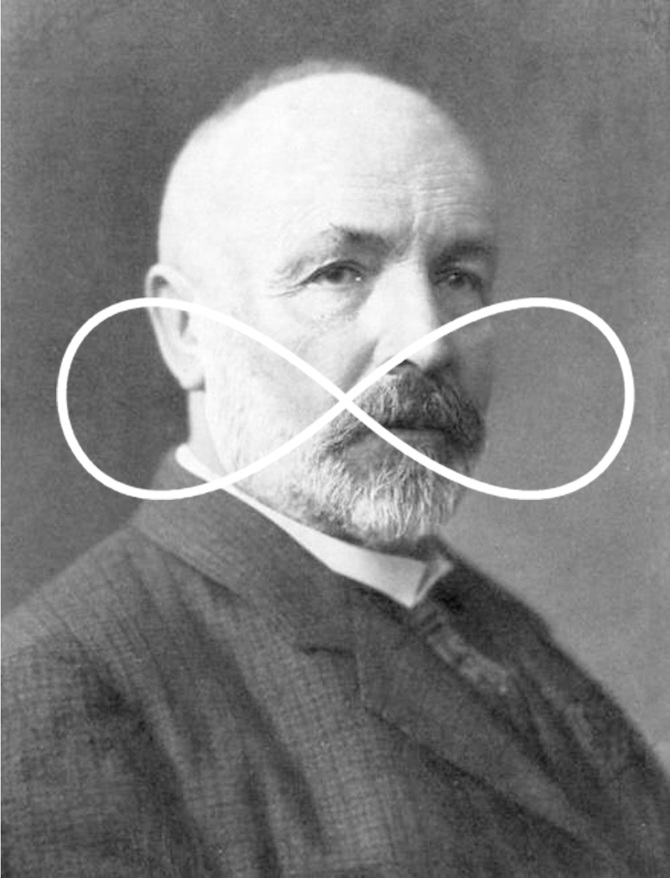
\includegraphics[scale = 0.25]{figs/cantor-infinity}} [counterclockwise from = 210]
	  child [] {node (nr) {$\mathbb{N}, \mathbb{R}$}}
	  child [] {node (cardinal) {$\aleph_{0}$}}
	  child [] {node (ordinal) {$\omega$}}
	}
    }
    child[] {
      node {Foundation of Mathematics \\ {\small (+ Logic)}} [counterclockwise from = -90]
	child [] {node (set) [] {$\{\}$} [
		counterclockwise from = 180, 
	        level 3 concept/.append style = {sibling angle = 60, font = \bfseries\LARGE, text width = 6em}]
	  child [] {node (pair) [font = \Huge] {$(a,b)$}}
	  child [] {node (cprod) [] {$A \times B$}}
	  child [] {node (relation) [] {$R \subseteq A \times B$}}
	  child [] {node (function) [] {$f: A \to B$}}
	}
    };
\end{tikzpicture}
\end{document}